\documentclass[12pt]{beamer}
\usetheme{Madrid}
\usecolortheme{default}

\usepackage{ragged2e}
\usepackage[utf8]{inputenc}
\usepackage[brazil]{babel}
\usepackage[T1]{fontenc}
\usepackage{amsmath}
\usepackage{amsfonts}
\usepackage{amssymb}
\usepackage{graphicx}
\usepackage{setspace}
\setbeamertemplate{caption}[numbered]
\usepackage{hyperref}
\setbeamercovered{transparent} 
\setbeamertemplate{navigation symbols}{}
\usepackage[table,xcdraw]{xcolor}
\usepackage{ragged2e}

%referência e citação
\usepackage[bibstyle=abnt-numeric,citestyle=authoryear,backend=biber,]{biblatex}
\addbibresource{ref.bib}

\addtobeamertemplate{block alerted}{}{\justifying}

\author[Joao Victor]{% 
	Joao Victor\inst{1} \and Joseph Cesar\inst{2} \and Everton de Souza\inst{3} \and Kauã Vidal\inst{4}}
\title[Planos de Amortização]{Empréstimos e Planos de Amortização}
\institute[]{% 	
	\textsuperscript{1,2,3,4} Graduando em Matemática
}
\titlegraphic{
\includegraphics[width=0.13\textwidth]{imagens/logo_3.jpg}}
\date{\today} 


\begin{document}
	\onehalfspacing 
	\justifying 
	
	\begin{frame}
		\titlepage
	\end{frame}
	
	\begin{frame}{Sumário}
		\tableofcontents
	\end{frame}
	
	\section{Introdução}
	
		\begin{frame}{Introdução}
			\justifying
			A matemática financeira está presente no cotidiano das pessoas, principalmente quando falamos sobre compras parceladas, financiamentos, cartões de crédito e empréstimos bancários.
		\end{frame}
	
		\begin{frame}{Introdução}
			\justifying
			Quando compramos uma casa, por exemplo, assinamos um contrato de hipoteca com uma instituição financeira (um banco, por exemplo). Nesse contrato, fica acordado que a instituição nos emprestará o dinheiro necessário para efetivar a compra do imóvel, em troca de pagamentos
			periódicos futuros.
		\end{frame}
		
		
		\begin{frame}{Introdução}
			\justifying
			Esses pagamentos possuem duas funções: parte deve pagar os juros correspondentes à atualização monetária da dívida e o restante serve para amortizar, ou seja, diminuir o saldo devedor original. A estrutura de pagamentos ao longo do tempo recebe o nome de sistema de amortização.
		\end{frame}
		
		\begin{frame}{Introdução}
			\justifying
			Ao longo deste material, abordaremos os dois tipos de
			sistema de amortização adotados no sistema financeiro brasileiro: o sistema \textit{Price} e o sistema de amortização constante (SAC). Porém, existem ainda o sistema americano,o sistema alemão e o sistema misto.
		\end{frame}
	
	
	\section{Principais Sistemas}
		
		\begin{frame}{Planos de Amortização - Principais Sistemas}
			
			\begin{columns}[T]
				
				\begin{column}{0.48\textwidth}
					\textbf{SAC – Sistema de Amortização Constante}
					\begin{itemize}
						\item A amortização é fixa;
						\item As parcelas diminuem com o tempo;
						\item Muito usado em financiamentos imobiliários.
					\end{itemize}
				\end{column}
				
				\begin{column}{0.48\textwidth}
					\textbf{Tabela Price (Sistema Francês)}
					\begin{itemize}
						\item Parcelas fixas;
						\item Juros maiores no início;
						\item Muito usada em financiamentos de veículos e lojas.
					\end{itemize}
				\end{column}
				
			\end{columns}
			
		\end{frame}
		
	\section{Vantagens e Desvantagens}
	
		\begin{frame}{Vantagens e Desvantagens - SAC}
			
			\begin{columns}[T]
				
				\begin{column}{0.48\textwidth}
					\textbf{Vantagens}
					\begin{itemize}
						\item Paga-se menos juros no total do contrato.
						\item A parcela fica cada vez mais barata, dando alívio no orçamento.
					\end{itemize}
				\end{column}
				
				\begin{column}{0.48\textwidth}
					\textbf{Desvantagens}
					\begin{itemize}
						\item As primeiras parcelas são bem mais altas, exigindo mais renda no começo.
					\end{itemize}
				\end{column}
				
			\end{columns}
			
		\end{frame}
		
		\begin{frame}{Vantagens e Desvantagens - Sistema Price}
			
			\begin{columns}[T]
				
				\begin{column}{0.48\textwidth}
					
					\textbf{Vantagens}
					\begin{itemize}
						\item Previsibilidade: você sabe exatamente quanto vai pagar todo mês.
						\item Parcelas iniciais mais acessíveis que as do SAC.
					\end{itemize}
				\end{column}
				
				\begin{column}{0.48\textwidth}
					\textbf{Desvantagens}
					\begin{itemize}
						\item Paga-se mais juros no total.
						\item A dívida cai muito devagar no início do contrato.
					\end{itemize}
				\end{column}
				
			\end{columns}
			
		\end{frame}
		
	\section{Aplicações}
	
		\begin{frame}{Financiamento SAC}
			\begin{exampleblock}{Exemplo 01.}
				\justifying
				Pedro tomou um empréstimo de R\$ 1000,00, a ser pago em 5 parcelas mensais, à taxa de juros de 10\% ao mês. Quais são os valores de cada parcela? Considere o Sistema SAC.
			\end{exampleblock}
		\end{frame}
		
		\begin{frame}{Financiamento SAC - Exemplo 01.}
			\begin{table}[h]
				\centering
				\begin{tabular}{|c|c|c|c|c|c|}
					\hline
					MÊS & DÍVIDA & AMORT & JUROS & PARCELA & SALDO \\
					\hline
					0 & - & - & - & - & 10000 \\
					\hline
					1 & & & & & \\
					\hline
					2 & & & & & \\
					\hline
					3 & & & & & \\
					\hline
					4 & & & & & \\
					\hline
					5 & & & & & \\
					\hline
				\end{tabular}
				\caption{Tabela SAC}
			\end{table}
		\end{frame}
		
		\begin{frame}{Financiamento Price}
			\begin{exampleblock}{Exemplo 02.}
				\justifying
				Pedro tomou um empréstimo de R\$ 1000,00, a ser pago em 5 parcelas mensais, à taxa de juros de 10\% ao mês. Quais são os valores de cada parcela? Considere o Sistema Price.
			\end{exampleblock}
		\end{frame}	
		
		\begin{frame}{Financiamento Price - Exemplo 02.}
		\begin{table}[h]
			\centering
			\begin{tabular}{|c|c|c|c|c|c|}
				\hline
				MÊS & DÍVIDA & AMORT & JUROS & PARC & SALDO \\
				\hline
				0 & & & & & 10000 \\
				\hline
				1 & & & & & \\
				\hline
				2 & & & & & \\
				\hline
				3 & & & & & \\
				\hline
				4 & & & & & \\
				\hline
				5 & & & & & \\
				\hline
			\end{tabular}
			\caption{Tabela Price}
		\end{table}
		\end{frame}
		
	\section{Sistema de Amortização Misto (SAM)}
	
		\begin{frame}{Sistema de Amortização Misto (SAM)}
			\justifying
			
			\begin{itemize}
				\justifying
				\item Cada prestação (pagamento) é a média aritmética das prestações respectivas no Sistemas Price e no Sistema de Amortização Constante (SAC). 
				
				\uncover<2->{
				\item Uso: Financiamentos do Sistema Financeiro da Habitação.
				}
			\end{itemize}

		\end{frame}
		
		\begin{frame}{Sistema de Amortização Misto (SAM)}
			\justifying
			
			Cálculo:
			
			$$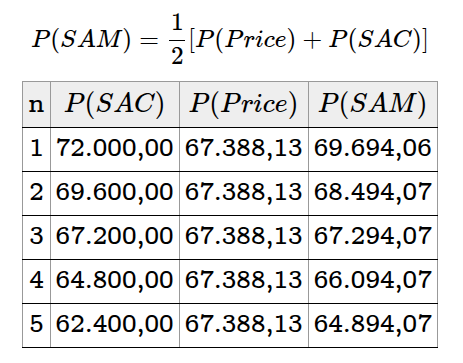
\includegraphics[scale=0.45]{imagens/sam.png}$$
		\end{frame}
		
		\begin{frame}{Sistema de Amortização Misto (SAM)}
			\justifying
			
			\begin{table}[h]
				\centering
				\begin{tabular}{|c|c|c|c|}
					\hline
					\textbf{Característica} & \textbf{Price} & \textbf{SAC} & \textbf{SAM} \\
					\hline
					Parcelas & Constantes & Decrescentes & Decrescentes\\
					\hline
					Primeira parcela & Média & Alta & Média-alta \\
					\hline
					Última parcela & Média & Baixa & Média-baixa \\
					\hline
					Juros totais & Maior & Menor & Intermediário \\
					\hline
				\end{tabular}
				\caption{Perfil das prestações}
			\end{table}
		\end{frame}
		
	\section{Sistema Americano}
	
		\begin{frame}{Sistema Americano}
			O devedor paga o Principal em um único pagamento no final e no final de cada período, realiza o pagamento dos juros do Saldo devedor do período. No final dos 5 períodos, o devedor paga também os juros do 5o. período.
		\end{frame}
		
		\begin{frame}{Sistema Americano}
			Sistema de Amortização Americano
			
			$$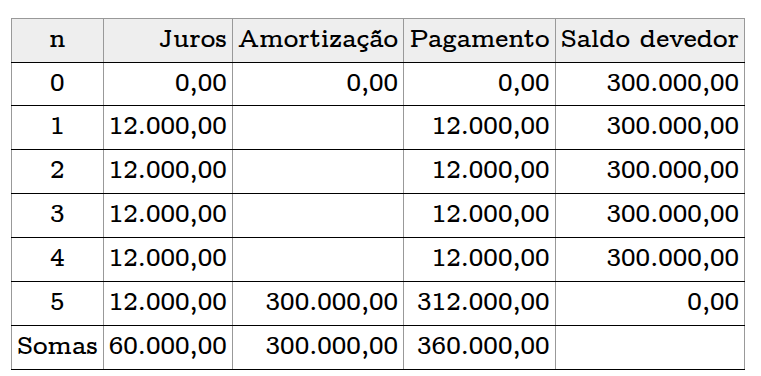
\includegraphics[scale=0.35]{imagens/sa.png}$$
		\end{frame}
		
		
	\section{Referências}
	
		\begin{frame}{Referências}
			
			\justifying
			\textit{SPINELLI, Walter; SOUZA, Maria Helena Soares de. Matemática Comercial e Financeira. 12. ed. São Paulo: Editora Ática, 2003.} 
			
			\vspace{2mm}
			
	
			
		\end{frame}
	
\end{document}